\section{REST}

REST ou Representational State Transfer é um estilo arquitetural usado para a comunicação de sistemas distribuídos através do protocolo HTTP. Foi introduzido por Roy Fielding em 2000 com o objetivo de oferecer às aplicações web um modelo de interface de acesso baseada em recursos. Além disso, descreve 6 tipos de restrições que serviços deveriam aplicar para ganho de performance, escalabilidade, simplicidade, modificabilidade, visibilidade, portabilidade e confiabilidade.

Vale lembrar que, por ter causado grande repercussão após sua publicação. O termo REST, segundo Richardson, acabou sofrendo diversas interpretações durante o tempo e, sua descrição representada de formas não originalmente propostas por Fielding. Alguns descrevem que serviços que violam essas restrições não podem ser considerados RESTful. Para Wildermuth, apesar de reconhecer as vantagens de cada restrição, serviços web devem usá-los de forma pragmatica. \cite{RichardsonEtAl2013} \cite{Wildermuth2015}

Apesar de ser introduzido num meio acadêmico, REST se adaptou bem em arquiteturas orientada a serviços. Segundo Pautasso, a eliminação da complexidade das soluções Web Services indicam que REST como uma solução aplicável para resolver problemas de integraçao de aplicaçoes empresariais e simplificar o encadeamento necessario para construir SOAs. A seguir, REST como adoção majoritária em relação a outros estilos para arquitetura de APIs. \cite{PautassoEtAl2008}

\begin{figure}[h]
  \centering
  \resizebox{\columnwidth}{!}{
    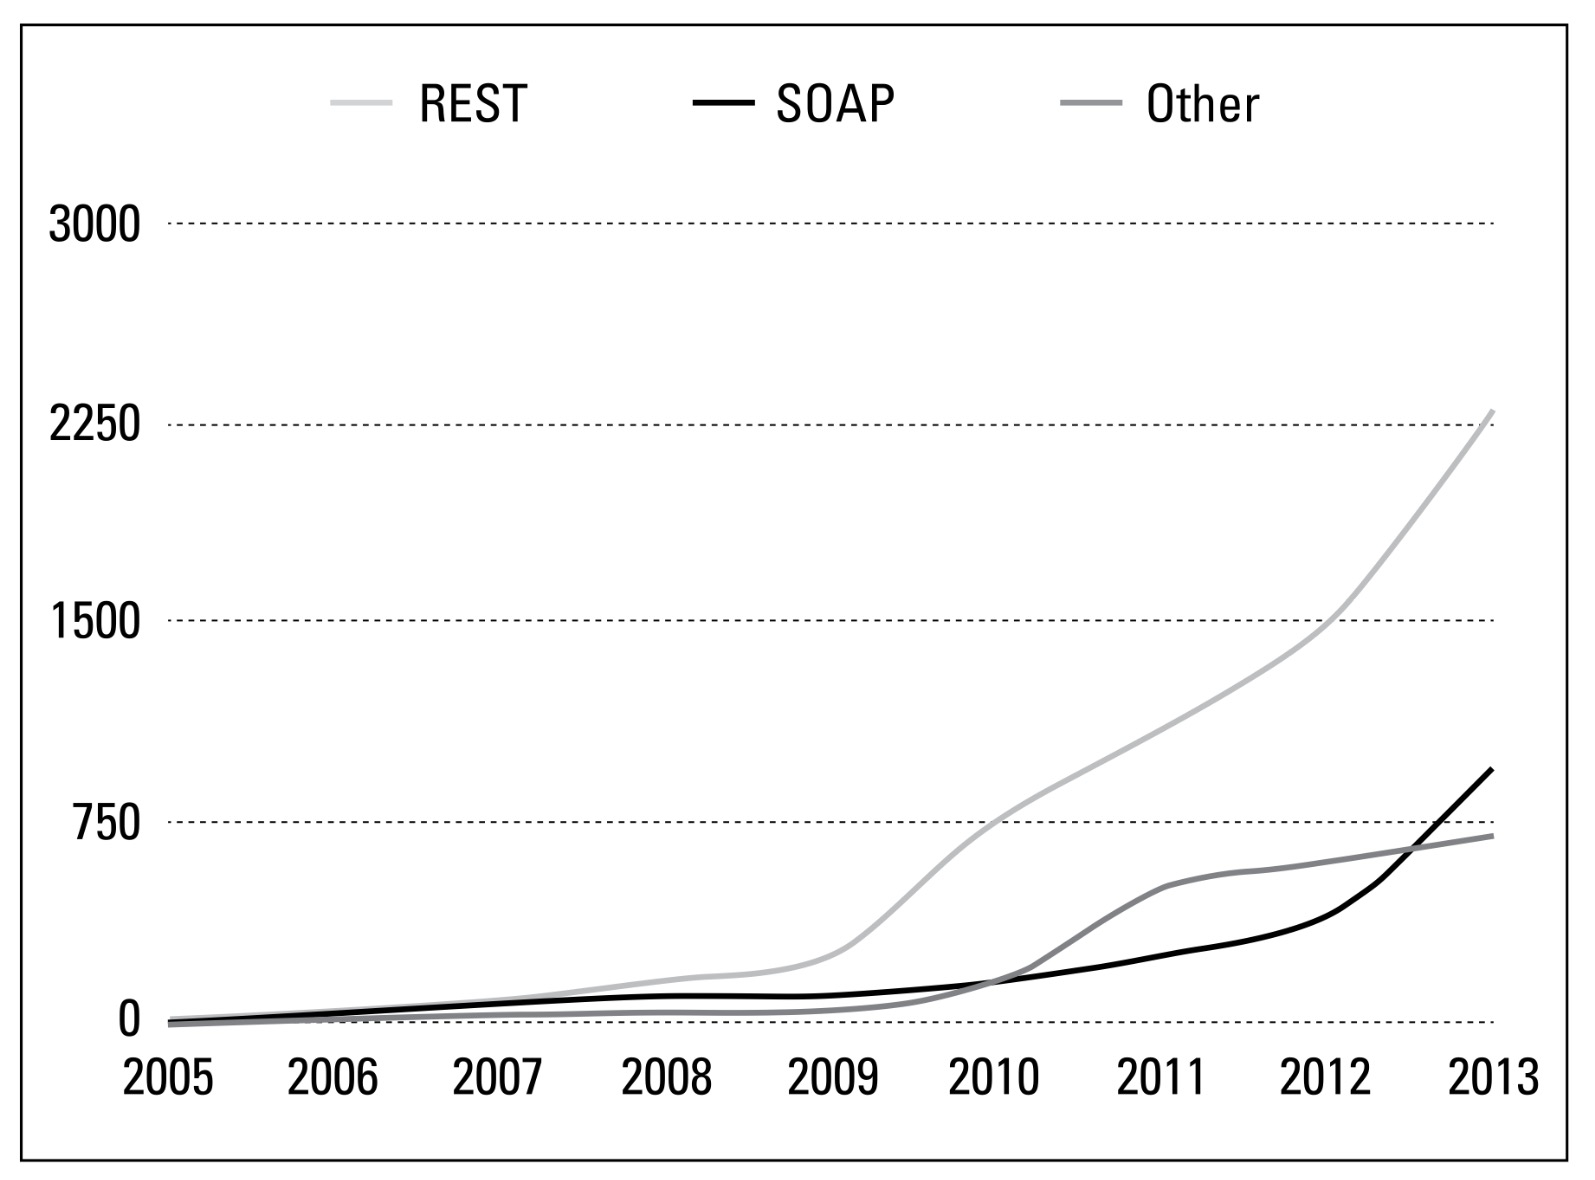
\includegraphics[width=\textwidth,height=\textheight,keepaspectratio]{figuras/api-styles.jpg}
  }
  \caption{Distribuição de estilos e protocolos para APIs}
\end{figure}

Sua maior vantagem de uso é por ser facilmente acessada por clientes web, mobile apps, dispositivos IoT. Isso permite que organizações construam clientes sem se preocupar com suporte à plataformas. Contudo, ao contrário de outros estilos de arquitetura, REST não sugere a criação de documentos de especificação, pois incentiva a escrita de respostas em hypertexo para navegação. Para Knupp, a idéia de documentação através de respostas autodescritivas dificulta a legibilidade, além de criar complexidade e informações adicionais. Ao invés, incentiva o uso de outras ferramentas de documentação e descrição de respostas. \cite{Knupp2016}

A seguir veremos sobre as restrições de arquitetura propostas pelo modelo REST, o que é uma API RESTful e seus níveis, além das atuais formas de documentação de APIs REST com suporte a leitura de máquinas.

\subsection[Restrições de Arquitetura]{Restrições de Arquitetura}

Esta seção fornece uma visão geral sobre as restrições propostas por Fielding para a implementação em arquiteturas web, além de ser examinado o impacto de cada restrição nesses sistemas distribuídos. \\

\textbf{Cliente-Servidor} \\

Nesta primeira restrição, não existe conexão entre cliente e servidor, mas sim a espera do servidor por pedidos de clientes através de chamada e resposta. O cliente (consumidor do serviço) não se preocupa com tarefas de comunicação de banco de dados, gerenciamento de cache, entre outros. Assim como o servidor (prestador de serviços) não está preocupado com as tarefas do cliente como interface ou experiência do usuário por exemplo. Permitindo a evolução independente dos dois ambientes, \textit{desde que sua interface de comunicação não seja alterada}. \cite{Fielding2000} \\

\textbf{Sem Estado} \\

Esta restrição ajuda na viabilidade, confiabilidade e escalabilidade de sistemas distribuídos, pois garantem que chamadas à API não estejam vinculadas a um determinado servidor. Como HTTP é um protocolo sem conexão, cada requisição deve conter todas as informações necessárias para que um servidor entenda o que um cliente está executando. Para Wildermuth, no entanto, dependendo da diversidade no número de clientes, ao manter um servidor sem estado, perder-se o controle no tamanho da estrutura de resposta necessária para atender a demanda de todos os clientes. \cite{Wildermuth2015} \\

\textbf{Interface Uniforme} \\

Em essência, Fielding propõe que aplicações façam o uso de verbos HTTP (POST, GET, PUT, DELETE) e identificadores uniforme de recursos (URI) para mapear operações em ambientes distribuidos e minimizar o acoplamento entre cliente-servidor. Essas regras de acesso são: \cite{Fielding2000}

\begin{itemize}[noitemsep]
\item Identificação de Recursos: Cada recurso deve ser disponibilizado através de uma URI específica e coesa. (Exemplo: GET /customers/1)
\item Manipulação de Recursos através de Representações: Um recurso pode ser representado em diferentes formatos para diferentes clientes. (Exemplo: HTML, XML, JSON)
\item Resposta Auto-explicativa: Metadados devem ser adicionados na requisição e resposta de um recurso para descrever seu estado atual ou desejado. (Exemplo: código de resposta HTTP, Host, Content-Type)
\item HATEAOS\footnote{
  Hypermedia as the Engine of Application State.
} - Caso um recurso possua relacionamentos, ao ser representado, estes devem estar especificados em forma de hiperlinks para facilitar a navegação de dados por clientes.
\end{itemize}

\textbf{Separação em Camadas} \\

Um dos princípios desta restrição está em evitar que clientes façam diretamente requisição para o servidor sem antes passar por um intermediário, como por exemplo um load balancer\footnote{
  Técnica para distribuir a carga de trabalho uniformemente entre dois ou mais computadores
}. Assegurando que clientes apenas se preocupem com a comunicação, deixando para que intermediários lidem com a distribuição de requisições. \cite{Fielding2000}

\begin{figure}[H]
  \centering  	   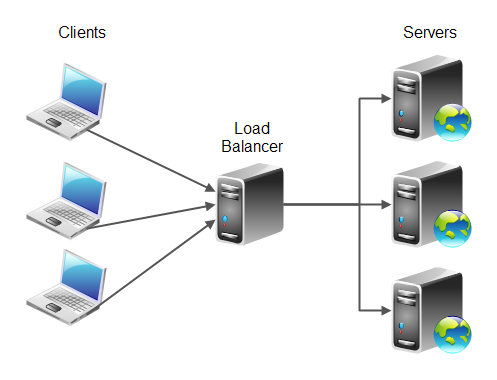
\includegraphics[width=0.7\textwidth,height=\textheight,keepaspectratio]{figuras/load-balancer.png}
  \caption{Exemplo de Load Balancer}
\end{figure}

\textbf{Código sob Demanda} \\

Apesar de ser a única restrição opcional do estilo, ela permite que servidores disponibilizem código em forma de script para que seja executado no cliente. Dessa forma, extendendo a lógica de serviço do servidor para seus clientes. \cite{Fielding2000} \\

\textbf{Cache} \\

Para aumentar desempenho de um serviço. Quando um recurso é acessado por mais de um cliente, se não houve mudança neste é recomendado que estas respostas sejam armazenadas em cache, evitando o processamento desnecessário. Isso significa que servidores, quando possível, devem implementar regras de cache para beneficio de ambos os ambientes. \cite{Fielding2000}

\subsection[RESTful]{RESTful}

Segundo Richardson, para que uma API de estilo REST seja consideirado RESTful, esta precisa seguir estritamente as regras exigidas anteriormente. Além disso, Richardson propõem uma escala de 4 níveis para avaliar a coesão e maturidade dessas APIs. \cite{RichardsonEtAl2013}

\begin{itemize}[noitemsep]
\item \textbf{Nível 0}: É a falta de qualquer regra; diz respeito ao uso de HTTP para operações de endereços no servidor. Normalmente, usa apenas um endpoint (URI) e um verbo HTTP.
\item \textbf{Nível 1}: Aplicação de recursos. A API é dividida em diferentes endpoints que indicam um ou mais recursos.
\item \textbf{Nível 2}: Implementação de verbos HTTP para diferentes tipos de operações. Onde uma mesma URI pode aceitar mais de um verbo para excução de diferentes procedimentos.
\item \textbf{Nível 3}: O conceito de HATEOS é aplicado para disponibilizar informações necessárias para interação e navegação da API.
\end{itemize}

\begin{figure}[H]
  \centering
  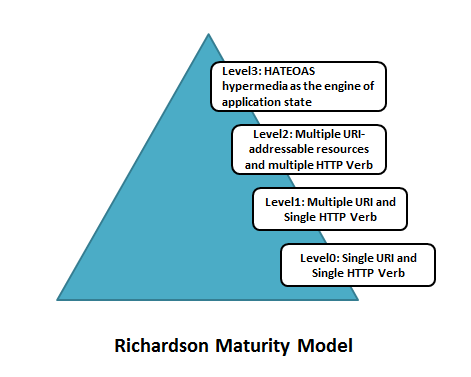
\includegraphics[width=0.8\textwidth,height=\textheight,keepaspectratio]{figuras/richardson-maturity-model.png}
  \caption{Modelo de Maturidade descrito por Richardson}
\end{figure}

\subsection[Descrições de API]{Descrições de API}

Em SaaS\footnote{
  Software as a Service.
}, APIs REST tornaram-se padrão como interface de acesso à serviços da empresa por seus clientes. A capacidade de oferer uma completa descrição sobre a api web para permitir que usuarios descubram e entam o serviço tornou-se critico para o sucesso da empresa. Contudo, apesar do processo de implementação tournou-se uma pratica comum, a definição de metadados de apis ainda não atingiu um grau de maturidade para normas amplamente aceitas. Apenas descrever manualmente APIs através de websites em linguagem natural permite que apenas pessoas entendam, isso se for bem projetada \cite{LuckyEtAl2016}

Com o fracasso de formatos tradicionais para descrição de web services como WADL, a adoção duvidosa de formatos hypermedia de resposta HATEOS como HAL e a demanda cada vez mais alta por boas especificações em formato legivel por humanos e maquinas. Nos últimos anos foram introduzidas diversas ferramentas e formatos de descrição para descrever Web APIs de REST, tanto em formatos legíveis para humanos como para máquinas. \cite{LuckyEtAl2016}

A seguir, comparações feitas por Sandoval entre as 3 linguagens mais usadas para especificação de APIs: \cite{Sandoval2015}

\begin{description}[leftmargin=8em,style=nextline]
  \item[\textbf{OpenAPI} (Swagger)] Pros: Amplamente adotada, grande comunidade, suporte pra diversas linguagens. \\ Cons: Carece de especificações de metadados mais avançadas.
  \item[\textbf{RAML}] Pros: Suporte a especificação avançada, adoção significativa, formato legível, bom suporte da indústria. \\ Cons: Falta de ferramentas de auxílio, não comprovada a longo prazo.
  \item[\textbf{API Blueprint}] Pros: Fácil de entender, simples de escrever \\ Cons: Pouca adoção, Carece de especificações de metadados mais avançadas, instalação complexa.
\end{description}

Recentemente, empresas como Heroku tem se dedicado ao uso do JSON Schema como formato de descrição de APIs, por ser uma tecnologia limpa e ainda pouco aplicada especificamente para a construção de grandes API \cite{Leach2014}. Já Lynn propõe um método de modelagem de REST API em serviços IoT utilizando JSON Hyper-Schema visto nos capítulos anteriores. Com suporte a descrição de entrada e saída de dados em toda a interface, junto com descrições URIs, relações e métodos que se aplicam aos links. Além disso, o formato suporta HATEOS e serve como entrada de documentação e ferramenta para geração de código. \cite{LynnEtAl2016}

